% !TEX root = figures-tables_subfile.tex

\chapter{Tables \& figures}

\section{Tables}

The class file provides custom macros \texttt{L}, \texttt{R} and \texttt{C} that can be used in conjunction with \texttt{tabularx} for automatic line wrapping within cells. Use the \texttt{S} to typeset numeric columns with \texttt{siunitx}.

\begin{table}[htbp]
    \centering
    \begin{tabularx}{0.6\linewidth}{lRS}
    \toprule
    \thead{Title 1} & \thead{Title 2} & \thead{Title 3} \\ \midrule
    Element 1 & Some text & 10.3546 \\
    Element 2 & A little more text over here & 2.543 \\
    Element 3 & A long line of text to test automatic line wrapping & 28.73 \\
   \bottomrule
\end{tabularx}
\caption{Simple table example}
\label{tab:simple-table}
\end{table}

\noindent Use \texttt{\textbackslash mcx} and \texttt{\textbackslash mrx} for multicolumn and multirow cells.

\begin{table}[htbp]
  \centering
  \begin{tabular}{lrrrr}
    \toprule
    \mrx{2}{\thead{Sample}} & \mcx{2}{I} & \mcx{2}{II} \\
    \cmidrule(lr){2-3} \cmidrule(lr){4-5}
      & A & B & C & D \\
    \midrule
    S1 & 5 & 8 & 12 & 2 \\
    S2 & 6 & 9 & 2 & 6 \\
    S3 & 7 & 9 & 5 & 8 \\
    S4 & 8 & 9 & 8 & 2 \\
    \bottomrule
\end{tabular}
\caption{Table with \texttt{\textbackslash mcx} and \texttt{\textbackslash mrx} macros}
\label{tab:mcx-mrx-macro}
\end{table}

Use the \texttt{longtable} environment (or \texttt{xltabular} if you want to provide the width of the table as an argument) to display tables across multiple pages.

\begin{xltabular}{\linewidth}{RRR}
  \caption{Example of longtable}\label{tab:longtable-example}\\
  \toprule
  {\thead{Title 1}} & {\thead{Title 2}} & {\thead{Title 3}} \\
  \midrule
  \endhead
  \midrule
  \multicolumn{3}{r}{\seenextpagename} \\
  \midrule
  \endfoot
  
  \bottomrule
  \endlastfoot
  One & abcdef ghjijklmn & 123.456778 \\
  One & abcdef ghjijklmn & 123.456778 \\
  One & abcdef ghjijklmn & 123.456778 \\
  One & abcdef ghjijklmn & 123.456778 \\
  One & abcdef ghjijklmn & 123.456778 \\
  One & abcdef ghjijklmn & 123.456778 \\
  One & abcdef ghjijklmn & 123.456778 \\
  One & abcdef ghjijklmn & 123.456778 \\
  One & abcdef ghjijklmn & 123.456778 \\
  One & abcdef ghjijklmn & 123.456778 \\
  One & abcdef ghjijklmn & 123.456778 \\
  One & abcdef ghjijklmn & 123.456778 \\
  One & abcdef ghjijklmn & 123.456778 \\
  One & abcdef ghjijklmn & 123.456778 \\
  One & abcdef ghjijklmn & 123.456778 \\
  One & abcdef ghjijklmn & 123.456778 \\
  One & abcdef ghjijklmn & 123.456778 \\
  One & abcdef ghjijklmn & 123.456778 \\
  One & abcdef ghjijklmn & 123.456778 \\
  One & abcdef ghjijklmn & 123.456778 \\
  One & abcdef ghjijklmn & 123.456778 \\
  One & abcdef ghjijklmn & 123.456778 \\
  One & abcdef ghjijklmn & 123.456778 \\
  One & abcdef ghjijklmn & 123.456778 \\
  One & abcdef ghjijklmn & 123.456778 \\
  One & abcdef ghjijklmn & 123.456778 \\
  One & abcdef ghjijklmn & 123.456778 \\
  One & abcdef ghjijklmn & 123.456778 \\
  One & abcdef ghjijklmn & 123.456778 \\
  One & abcdef ghjijklmn & 123.456778 \\
  One & abcdef ghjijklmn & 123.456778 \\
  One & abcdef ghjijklmn & 123.456778 \\
  One & abcdef ghjijklmn & 123.456778 \\
\end{xltabular}

\section{Figures}

Use the \texttt{subfigure} environment for subfigures.

\begin{figure}[htbp]
    \centering
    \begin{subfigure}[t]{0.47\linewidth}
        \centering
        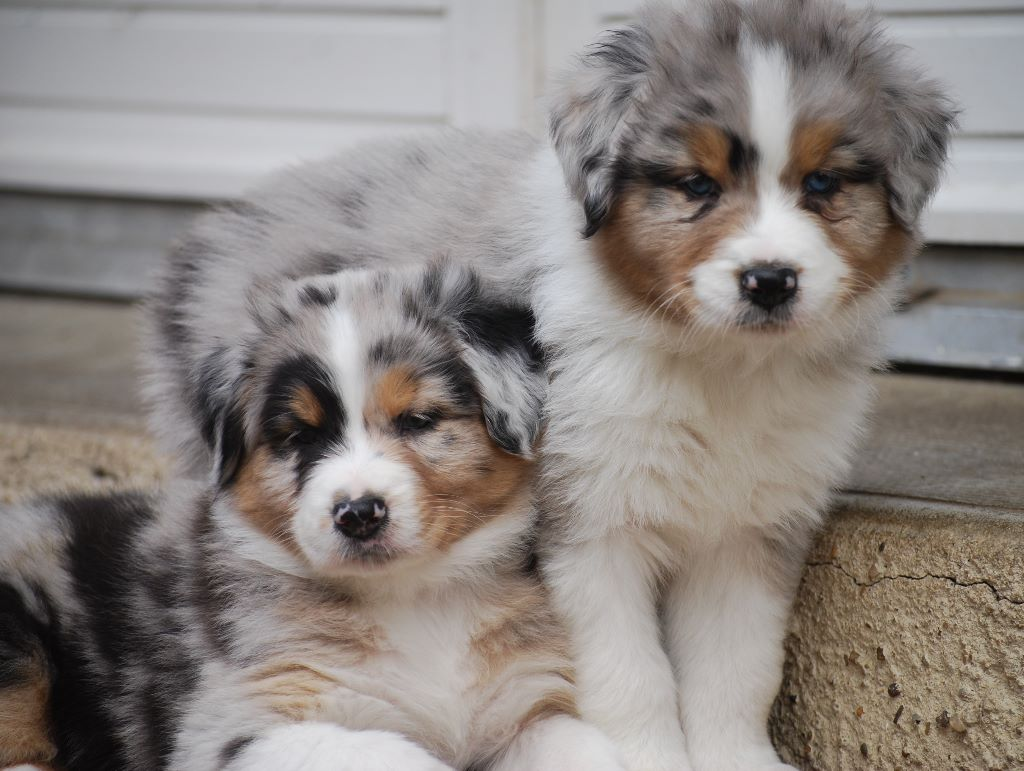
\includegraphics[height=4.3cm]{figs/img1}
        \caption{Image 1}
    \end{subfigure}
    ~
    \begin{subfigure}[t]{0.47\linewidth}
        \centering
        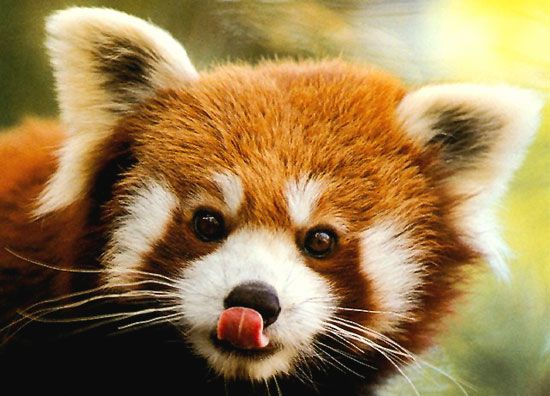
\includegraphics[height=4.3cm]{figs/img2}
        \caption{Image 2}
    \end{subfigure}
\caption{An example of subfigure}
\end{figure}
